\begin{frame}[t, label=gen_pop]
    \frametitle{\alert{Step 1:} Generate Meteor Population}
    % top right graphic
    \begin{textblock*}{2cm}(\paperwidth-2.05cm, 0.05cm)
        \raggedleft 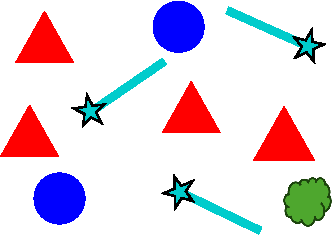
\includegraphics[height=1cm]{img/gen_sim.pdf}
    \end{textblock*}
    % GIP and distributions
    \begin{tikzpicture}[remember picture, overlay]
        \node[anchor = east] (img) at ([xshift=0cm, yshift=-1cm]current page.east) { 
            \adjincludegraphics[width=0.7\pagewidth, trim={0 {.2\height} {0.01\width} {.22\height}},clip]{img/GIP_expect.pdf}
        };
        \node<3>[anchor = north east] at ([yshift=0.75cm]img.north east) { 
            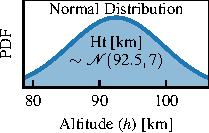
\includegraphics[width=0.25\linewidth]{img/param_distributions/ht_normal_pdf.pdf}
        };
        \node<4>[anchor = north east] at ([yshift=0.75cm]img.north east) { 
            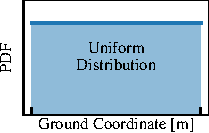
\includegraphics[width=0.25\linewidth]{img/param_distributions/gnd_uniform_pdf.pdf}
        };
        \node<5>[anchor = north east] at ([yshift=0.75cm]img.north east) { 
            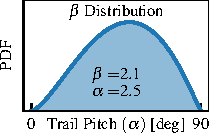
\includegraphics[width=0.25\linewidth]{img/param_distributions/alpha_beta_pdf.pdf}
        };
        \node<6>[anchor = north east] at ([yshift=0.75cm]img.north east) { 
            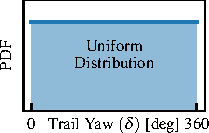
\includegraphics[width=0.25\linewidth]{img/param_distributions/delta_uniform_pdf.pdf}
        };
        \node<7>[anchor = north east] at ([yshift=0.75cm]img.north east) { 
            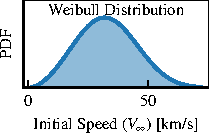
\includegraphics[width=0.25\linewidth]{img/param_distributions/speed_weibull_pdf.pdf}
        };
        \node<8>[anchor = north east] (dist) at ([yshift=0.75cm]img.north east) { 
            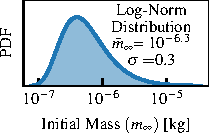
\includegraphics[width=0.25\linewidth]{img/param_distributions/mass_lognorm_pdf.pdf}
        };
        \node<9>[anchor = center] at (dist.center) { 
            {\(q_e = \frac{4}{9} \frac{ m_{\infty} \beta(V_{\infty})}{\overline{\mu}_{{A}}H}\sin(\alpha)\)}
        };
        \node<10>[anchor = center] at (dist.center) { 
            {\(l_{\parallel} = H \csc(\alpha)\)}
        };
        \node<11>[anchor = north east] at ([yshift=0.75cm]img.north east) {
            \begin{minipage}{0.25\linewidth}
                \begin{align*}
                    & l_\perp  = \\ & 6.54 \times 10^{16} \frac{V_\infty^{0.8}}{n_a} 
                \end{align*}
            \end{minipage} 
        };
        \node<12>[anchor = north east] at ([yshift=0.75cm]img.north east) {
            \begin{minipage}{0.25\linewidth}
                \begin{tcolorbox}[width = \linewidth, boxrule=0pt,colback=yellow,arc=0pt,outer arc = 0pt,left=1pt,right=1pt,boxsep=1pt, top=1pt, bottom=1pt]
                    \raggedright
                    \textbf{7 stocastic variables total}
            \end{tcolorbox}
            \end{minipage} 
        };
    \end{tikzpicture}
    \begin{minipage}{5cm}
        \begin{tcolorbox}[width=5cm, halign=center,  boxrule=1pt, arc=0pt,auto outer arc,left=0pt,right=0pt,boxsep=0pt]
           A \alert{single meteor} can be described by just \alert{a few characteristics}
    \end{tcolorbox} %         
    \end{minipage}
    %
    \uncover<2->{$\longrightarrow$ %
    %
    \begin{minipage}{5cm}
        \begin{tcolorbox}[width=5cm, halign=center,  boxrule=1pt, arc=0pt,auto outer arc,left=0pt,right=0pt,boxsep=0pt]
        A \alert{population of meteors} is generated by \alert{sampling these characteristics} 
    \end{tcolorbox}
    \end{minipage}} \hfill
    %
    \vspace{1.2\baselineskip}
    %
    \begin{columns}
        \begin{column}{0.45\textwidth}
            Geometric characteristics
            {\setlength{\leftmargini}{1em} \footnotesize
            \begin{itemize}
                \item<alert@3> \alert<12>{Altitude} \visible<12>{(\(h\))}
                \item<alert@4> \alert<12>{Ground coordinate} \visible<12>{(east, north)}
                \item<alert@5> \alert<12>{Trail orientation: pitch} \visible<12>{(\(\alpha\))}
                \item<alert@6> \alert<12>{Trail orientation: yaw} \visible<12>{(\(\delta\))}
            \end{itemize}}
            Physical characteristics
            {\setlength{\leftmargini}{1em} \footnotesize \begin{itemize}
                \item<alert@7> \alert<12>{Initial speed} \visible<12>{(\(V_{\infty}\))}
                \item<alert@8> \alert<12>{Initial mass} \visible<12>{(\(m_{\infty}\))}
                \item<alert@9> Maximum electron line density %(\(q_e\))
                \item<alert@10> Trail correlation length %(\(l_{\parallel}\))
                \item<alert@11> Trail radius %(\(l_{\perp}\)) 
            \end{itemize}}
        \end{column}
        \begin{column}{0.6\textwidth}
            
        \end{column}
    \end{columns} 
    
\end{frame}
